\chapter{The Forward Model}
\label{ch:formodel}
\thispagestyle{empty}

In this Chapter, we present the forward model to which we apply our entire methodology.
A singular value analysis for different measurement scenarios is conducted to understand the forward model and to determine a sensible way to measure the ozone concentration in the atmosphere. We follow the MIPAS handbook~\cite{mipas2000handbook} and simulate data according to an idealised cloud-free atmosphere in local thermodynamic equilibrium, assuming a measurement instrument with infinite spectral resolution and no pointing errors.
This is a simplified forward model.
No other instrument-specific details such as sensor area or antenna response are included because they are not available to us. 

\begin{figure}[ht!]
	\centering
	\input{LIMB.pdf_tex}
	\caption[Schematic of measurement and analysis geometry.]{Schematic of measurement and analysis geometry, not to scale.
		The stationary satellite, at a constant height $h_\text{sat}$ above Earth, takes $m$ measurements along its line-of-sight defined by the line $\Gamma_j$.
		Each measurement has a pointing angle $\phi_j$ and a tangent height $h_{\ell_j}$, $j=1,2,\dots,m$ defined as the closest distance of $\Gamma_j$ to the Earth's surface.
		Between $h_{L,0} \approx 7$km and $h_{L,n} \approx 83$km, the atmosphere is discretised into $n$ layers as illustrated by the solid green lines.}
	\label{fig:LIMB}
\end{figure}
As displayed in Fig.~\ref{fig:LIMB}, a satellite at a constant height $h_{\text{sat}}$ is pointing through the atmosphere (limb-sounding) to measure thermal radiation of ozone.
For each measurement $j=1,2,\ldots,m$, the tangent height $h_{\ell_j}$ and the corresponding line-of-sight $\Gamma_j$ are defined.
Additionally, we introduce the pointing angle $0 \leq \phi_j < \phi_{\text{max}}$, so that if $\phi = 0 \text{arc sec}$ the satellite points at $h_{L,0}$ and for a pointing angle $\phi_{\text{max}}$ at $h_{L,n}$.
The pointing angle is helpful to describe the measurement test cases in Sec.~\ref{sec:SVD}.
Further, the atmosphere is discretised into $n$ layers defined by height values $h_{L,i-1} < h_{L,i}$ with respect to the surface of the Earth, for $i = 1, \dots, n$.
More specifically, the $i$-th layer is defined by two spheres around the centre of the Earth with radii $ r_0 + h_{L,i-1} $ and $r_0 + h_{L,i}$, where $r_0$ is the Earth's radius.
Within a layer the signal is constant, whereas above $h_{L, n}$ and below $h_{L,0} $ no signal can be obtained.


\section{Radiative Transfer Equation}
\label{sec:RTE}
One noise-free measurement of thermal radiation emitted by gas molecules within the atmosphere is described by the radiative transfer equation (RTE)~\cite{mipas2000handbook}
\begin{align}
	\label{eq:RTE} 
	  \int_{\Gamma_j}  B(\nu,T) k(\nu, T)   \frac{p(r)}{k_{\text{B}} T(r)}  x(r)  \tau(r) \text{d}r \,  \\
\text{with} \,	\tau(r) = \exp{ \Bigl\{ - \int^{r}_{r_\text{obs}}  k(\nu, T)   \frac{p(r^{\prime})}{k_B T(r^{\prime})}  x(r^{\prime}) \text{d}r^{\prime} \Bigr\} } \, \label{eq:absRTE} .
\end{align}
This is a path integral along the satellite's straight line of sight $\Gamma_j$ with the ozone volume mixing ratio (VMR) $x(r)$ at distance $r$ from the satellite, at the wave number $\nu$.
Within the atmosphere, the number density $p(r) / (k_{\text{B}} T(r))$ of molecules is dependent on the pressure $p(r)$, the temperature $T(r)$, and the Boltzmann constant $k_{\text{B}}$.
The factor $\tau(r)\leq 1$ accounts for re-absorption of the radiation along the line-of-sight, which makes the RTE non-linear.
The absorption constant is given as
\begin{align}
	k(\nu, T) = L(\nu, T_{\text{ref}}) \frac{Q(T_{\text{ref}})}{Q(T)} \frac{ \exp{\{ - c_2 E^{\prime \prime} / T\}} }{\exp{\{ - c_2 E^{\prime \prime} / T_{\text{ref}} \}}} \frac{ 1- \exp{\{ - c_2 \nu  / T \}} }{1 - \exp{\{ - c_2 \nu / T_{\text{ref}} \}}}
\end{align}
with Planck's constant $h$ and speed of light $c$.
The line intensity $L(\nu, T_{\text{ref}})$ at reference temperature $T_{\text{ref}} =296K $, the lower-state energy $ E^{\prime \prime} $ in $\text{cm}^{-1}$ of the targeted transition and the second radiation constant $c_2\coloneqq hc/k_{\text{B}} \approx 1.44\text{cmK}$ are provided by the HITRAN database~\cite{gordon2022hitran2020}.
The total internal partition function is given as
\begin{align}
	Q(T )= g^{ \prime} \exp{\{ - \frac{ c_2 E^{ \prime} }{T}\}} + g^{\prime \prime} \exp{\{ - \frac{ c_2 E^{\prime \prime} }{T}\}} \, ,
\end{align}
with the statistical weight $ g^{\prime \prime}$ for the lower and $ g^{ \prime}$ for the upper energy state (also called the degeneracy factors) accounting for the molecule's non-rotational and rotational energy states (see also~\cite{vsimevckova2006einstein}), and the upper state energy $E^{ \prime} = E^{ \prime\prime} + \nu$.
Under the assumption of local thermodynamic equilibrium (LTE), the black body radiation acts as a source function
\begin{align}
	B(\nu,T)   = \frac{2 h c^2 \nu^3}{\exp{\{\frac{c_2\nu}{ T}\}}-1}\, .
\end{align}
For fundamentals on the RTE, we recommend~\cite[Chapter 1]{rybicki2000rte}, and for a more comprehensive model, we refer to \cite{read2006forwardModel}.

When simulating data, we assume an idealised limb-sounder.
Since the measurement device has a negligible frequency window, we neglect line broadening around $\nu$ for the calculations of $L(\nu, T_{\text{ref}})$.
Normally, this is modelled as the convolution of the normalised Lorentz profile (collisional/pressure broadening) and the normalised Doppler profile (thermal broadening)~\cite{mipas2000handbook}.
Additionally, we target one specific molecule and calculate $k(\nu, T)$ accordingly.
Usually, this would involve a summation over the individual absorption constants for multiple radiating molecules weighted by their respective VMR~\cite{mipas2000handbook}.


\section{Simulated Data and Ground Truth}
\label{sec:SimDat}
As the ground truth for our methodology, we consider an ozone profile at distinct pressure values generated from some data~\cite{MLSdata} of the MLS on the Aura satellite within the Antarctic region.
This ozone profile has a peak in the middle atmosphere and a second peak at higher altitudes, see Fig.~\ref{fig:O3Samp}, which seems to be a typical nighttime profile~\cite{Lee2020NightOzone}.
For more information on the processes within the atmosphere for ozone, we refer to~\cite{Lee2020NightOzone}.

We can relate the height $h$ and the pressure values $p$ via the hydrostatic equilibrium equation
\begin{align}
	\text{d}(\log p) = \frac{\text{d}p}{p} = \frac{- g M}{R^* T} \text{d} h \, .\label{eq:hydr}
\end{align}
Here the acceleration due to gravity is $g$, the universal gas constant is $R^* = 8.31432 \times 10^{-3} \text{Nm} / \text{kmol} / \text{K}$ and the mean molecular weight of the air is $M = 28.97 \text{kg/kmol}$, as in~\cite{atmosphere1976us}.
To enable efficient calculation of the RTE we discretise the atmosphere as in Fig.~\ref{fig:LIMB}.
Then the ozone VMR $\bm{x} =\{x_1,x_2,\ldots,x_n\} \in \mathbb{R}^{n}$, pressure $\bm{p} =\{p_1,p_2,\ldots,p_n\} \in \mathbb{R}^{n}$ and temperature $\bm{T} =\{T_1,T_2,\ldots,T_n\} \in \mathbb{R}^{n}$, as well as all other height dependent parameters, are discretised profiles with constant values between the heights $h_{L,i-1} \leq h < h_{L,i}$, for each layer $i = 1,\dots, n$.
The hydrostatic equilibrium equation for the discretised atmosphere is
\begin{align}
	h_{L,i+1} =  h_{L,i} - \frac{\Delta p R^* T_i  }{p_i  g_i M} \, 
\end{align}
with $\Delta p = p_{i+1} - p_{i}$ and $T_i = T(h_i)$ as in Eq.~\ref{eq:tempFunc} (see also~\cite{Carlotti99,Ridolfi00}).
At sea level $h_0 = 0$km the mean pressure is $p_0 = 1013.25$hPa and the mean temperature is $T_0 = 288.15$K~\cite{atmosphere1976us}.
The acceleration due to gravity is
\begin{align}
	g_i = g_0 \Bigg( \frac{r_0}{r_0 + h_{L,i}} \Bigg) \, ,
\end{align}
where the polar radius of the Earth is $r_0 \approx 6356 \, \text{km}$, the gravitation at sea level is $g_0 \approx 9.81 \text{m}/\text{s}^2$.
For a ground truth temperature profile (see Fig.~\ref{fig:PriorTemp}), we follow~\cite{atmosphere1976us} and form the temperature function
\begin{equation}
	\label{eq:tempFunc}
	T(h) = \adjustbox{max width=0.825\textwidth}{$\begin{dcases*}
			T_0 &, \text{$h  = 0$}\\
			T_0 + a_0 h   &, \text{$0 \leq h < h_{T,1}$}\\
			T_0 + a_0 h_{T,1} &, \text{$h_{T,1} \leq  h < h_{T,2}$}\\
			T_0 + a_0 h_{T,1} + a_1 (h_{T,2}   - h_{T,1})  + a_2 (h   - h_{T,2})  &, \text{$h_{T,2} \leq h < h_{T,3}$}\\
			T_0 + a_0 h_{T,1} + a_1 (h_{T,2}   - h_{T,1})   & \\
			\hphantom{{} T_0 } + a_2 (h_{T,3}   - h_{T,2}) + a_3 (h   - h_{T,3}) &, \text{$h_{T,3} \leq h < h_{T,4}$}\\
			T_0 + a_0 h_{T,1} + a_1 (h_{T,2}   - h_{T,1})  & \\
			\hphantom{{} T_0 }+ a_2 (h_{T,3}   - h_{T,2})  + a_3 (h_{T,4}   - h_{T,3}) + a_4 (h   - h_{T,4}) &, \text{$h_{T,4} \leq h < h_{T,5}$}\\
			T_0 + a_0 h_{T,1} + a_1 (h_{T,2}   - h_{T,1})   & \\
			\hphantom{{} T_0 } + a_2 (h_{T,3}   - h_{T,2}) + a_3 (h_{T,4}   - h_{T,3}) + a_4 (h_{T,5}   - h_{T,4})& \\
			\hphantom{{} T_0 }  + a_5 (h   - h_{T,5}) &, \text{$h_{T,5} \leq h < h_{T,6}$}\\
			T_0 + a_0 h_{T,1} + a_1 (h_{T,2}   - h_{T,1})    &\\
			\hphantom{{} T_0}  + a_2 (h_{T,3}   - h_{T,2}) + a_3 (h_{T,4}   - h_{T,3}) + a_4 (h_{T,5}   - h_{T,4}) &\\ 
			\hphantom{{} T_0} + a_5 (h_{T,6}   - h_{T,5}) + a_6 (h   - h_{T,6})   &, \text{$h_{T,6} \leq h \lesssim  86$}
		\end{dcases*}$}\\
\end{equation}
with gradient and height values in Tab.~\ref{tab:tempGrad} provided by~\cite{atmosphere1976us}.
This holds up to a geometric height of $86$km, where we ignore a $0.04\%$ non-linear change in $M$ from $80$km to $86$km.
\begin{table}
	\centering
	\begin{tabular}{ |c||c|c|  }
		\hline
		subscript $i$ & geometric height $h_{T,i}$ in km&gradient $a_i$\\
		\hhline{|=||=|=|}
		0& 0 & -6.5\\
		1& 11 & 0\\
		2& 20.1& 1\\
		3& 32.2& 2.8\\
		4& 47.4& 0\\
		5& 51.4& -2.8\\
		6& 71.8& -2\\
		\hline
	\end{tabular}
	\caption[Height depending temperature gradients]{Definition of height depending temperature gradients.}
	\label{tab:tempGrad}
\end{table}

We target ozone at a frequency of $235.71$GHz, which lies within the region where the MLS observes ozone~\cite{livesey2008ozonecarbonmono, waters2006earth}.
The corresponding wave number is $\nu = 7.86\text{cm}^{-1}$.
The absorption constant $k(\nu,T)$ is calculated as in Eq.~\ref{eq:absRTE}, following the high-resolution transmission (HITRAN) database~\cite{gordon2022hitran2020}.
The HITRAN database provides the line intensity $L(\nu,T_{\text{ref}})$ for the isotopologue $\prescript{16}{}{\text{O}}_3$ with the AFGL Code 666.

To compute a data vector, we define an atmosphere between $h_{L,1} = 6.9$km and $h_{L,n} = 83.3$km with $n = 45$ equidistant layers and a satellite fixed at a height of $h_{\text{sat}} = 500$km (see Fig.~\ref{fig:LIMB}).
The integrals in Eq.~\ref{eq:RTE} and Eq.~\ref{eq:absRTE} are evaluated using the trapezoidal rule and define the non-linear forward model $\bm{A}(\bm{x},  \bm{p},\bm{T})   \in \mathbb{R}^{m}$ for a set of $m$ noise-free measurements.
Here, each entry $A_{j}$ of $\bm{A}(\bm{x},\bm{p},\bm{T})\in \mathbb{R}^{m}$ includes multiple evaluations of the integral in Eq.~\ref{eq:absRTE} to calculate the absorption $\tau(r)$.
For brevity we denote the non-linear forward model as $\bm{A}(\bm{x}) \coloneqq \bm{A}(\bm{x},  \bm{p},\bm{T})$.
The simulated data vector
\begin{align}
	\bm{y} = \bm{A}(\bm{x}) + \bm{\eta}\, 
\end{align}
includes an additive identically-distributed Gaussian noise vector $\bm{\eta} \sim \mathcal{N}(0,\gamma^{-1} \bm{I})$.
The noise precision is chosen so that the signal-to-noise ratio (SNR) is approximately $150$.
The SNR is defined as
\begin{align}
	\text{SNR} \coloneqq \frac{\max(y)}{\text{STD noise}} = \frac{\text{peak signal}}{\text{RMS noise}} \label{eq:SNR} \, ,
\end{align}
where STD noise is the standard deviation of the noise.
An SNR of 150 is similar to~\cite{Froidevaux2008snrozone}, where a signal with a maximal spectral intensity of around $100\text{K}$ and a noise range of $0.4$ to $1.6\text{K}$ is reported.

By neglecting the absorption (e.g., set $\tau = 1$ in Eq.~\eqref{eq:absRTE}) the RTE is linearised.
This denotes the linear forward model matrix $\bm{A}_L\in \mathbb{R}^{m\times n}$.
The integral in Eq.~\eqref{eq:RTE} is evaluated using the trapezoidal rule and enables matrix-vector multiplication $\bm{A}_L \bm{x}$ to compute noise-free linear data.
Since neglecting the absorption changes the measurements only slightly (about $1\%$, see Chapter~\ref{ch:affine}), we classify the inverse problem as a weakly non-linear inverse problem.
Note that the methods used in this thesis will work with different SNRs or other frequencies.




%Note that, since we aim to provide estimates over pressure $\bm{p}$ and temperature $\bm{T}$, we explicitly include them as parameters in our forward model.
%This gives us a non-linear forward model matrix $\bm{A}_{NL} = \bm{A}(\bm{x}, \bm{p}, \bm{T}) \in \mathbb{R}^{m \times n}$, where $\bm{x}\in \mathbb{R}^{n}$ is vector related to the ozone VMR, $\bm{p}\in \mathbb{R}^{n}$ is the vector describing the pressure values and $\bm{T}\in \mathbb{R}^{n}$ the temperature values.
%The gradients and heights are chosen according to the different layers within the atmosphere


\subsection{Singular Value Decomposition of the Linear Forward Model}
%\textcolor{red}{understanding the forward map}
\label{sec:SVD}
In this section, we conduct a singular value decomposition (SVD) for the linear forward model and test for five different measurement strategies.

An SVD of the forward model matrix provides a quick and intuitive way of assessing the information provided by the forward model and if the data collection is effective.
More specifically, the behaviour of the singular values tells us how much information is passed through the forward model and how the measurement strategy affects that information.
The SVD of the linear forward model matrix $\bm{A}_L \in \mathbb{R}^{m \times n}$ is given as
\begin{align}
	\bm{A}_L = \sum_{j =1}^{r} \bm{u}_j  \sigma_j \bm{v}^T_j = \bm{U} \bm{\Sigma} \bm{V}^T
\end{align}
with $r = \min\{m,n\}$.
Our main objective is to measure ozone $\bm{x}$, so this forward model $\bm{A}_L$ includes temperature and pressure.
The pressure is dominant, see Fig.~\ref{fig:PriorPressOverTemp}, decreases exponentially in height and affects the information passed through the model.
If the pressure is high, the signal is large.
If the pressure is low, the signal is low, and the data tends to be noise-dominated.
%\textcolor{red}{The action of A on the paraemter
%Information about the projection of f along vk is “encoded” in the data as the component
%along the direction uk . The size of the projection is multiplied by sigma k to give the coefficient of
%uk , namely sigma k fk . The singular value is the factor which tells us by how much each component
%defining the image is amplified or attenuated when it is converted into the data
%not be changed in any way. If we now think of solving the inverse problem of reconstructing
%f from a measurement of d, it is clear that at best, those components of f along the first r
%right singular vectors are determined by the data. However the data tell us nothing at all
%about the components of f along the remaining n - r right singular vectors, and we have to
%use some other means for determining these components.}

The SVD of the forward model $\bm{A}_L$ provides information on how the right singular vectors $\bm{v}_i$ act on the parameter $\bm{x}$, because a noise-free measurement vector is given as~$\bm{A}_L\bm{x}$.
The singular values $\sigma_j $, ordered in size from the largest $\sigma_1$ to the smallest~$\sigma_{r}$, weigh that information from the right singular vectors to the left singular vectors~$\bm{u}_j$.
The left singular vectors project $\sigma_j \bm{v}^T_j \bm{x} $ onto the data space.
For a large singular value the forward model is informative about parameter structures represented by the corresponding right singular vector. 
For a small singular value the forward model is uninformative about parameter structures represented by the corresponding right singular vector.
%\textcolor{red}{WQhat is the vice versa? Not clear what you are saying. }
%Note that we obtain the same results using the non-linear forward model $\bm{A}(\bm{x})$ to do this analysis, where we would rewrite to the matrix-vector multiplication $\bm{A}_{NL} \bm{x}$, where $\bm{A}_{NL}$ is depend on $\bm{x}$.

Based on the assumption that the largest singular value $\sigma_1  \approx \max(y)$ as in Eq.~\ref{eq:SNR}, then most of the information transmitted through the forward model corresponds to the singular values $\sigma_j \gtrsim \max(y)/ \text{SNR}$~\cite{fox2025BlokkLecNot}.
For very small singular values $\sigma_j \ll \sigma_1/\text{SNR}$ below the RMS noise level or the noise STD, an effective rank $r_{\text{eff}} \leq r$ is introduced and the data space spanned by $ \{\bm{u}_{r_{\text{eff}} +1}, \dots ,\bm{u}_r \}$ is noise-dominated.
We say a forward model matrix is informative if it has a large effective rank and the singular values decrease gradually.
If the effective rank is small and the singular values decrease quickly, we classify this forward model as uninformative.

For large singular values above the SNR the associated data space is hardly influenced by the noise.
Therefore, reconstructions in the parameter space spanned by the respective right singular vectors are expected to be close to the ground truth.
For singular values around the SNR the noise is starting to influence the data space.
Hence, reconstructions in the parameter space spanned by the corresponding right singular vectors are expected to have increasing uncertainties.
Reconstructed parameter values in the parameter space spanned by $ \{\bm{v}_{r_{\text{eff}} +1}, \dots ,\bm{v}_r \}$ (e.g.~in Fig.~\ref{fig:nullSpace}) are expected to have large errors and to be determined by the prior because they relate to very small singular values.
See~\cite{tan2016LecNot} for a more comprehensive analysis.

\begin{figure}[ht!]
	\centering
	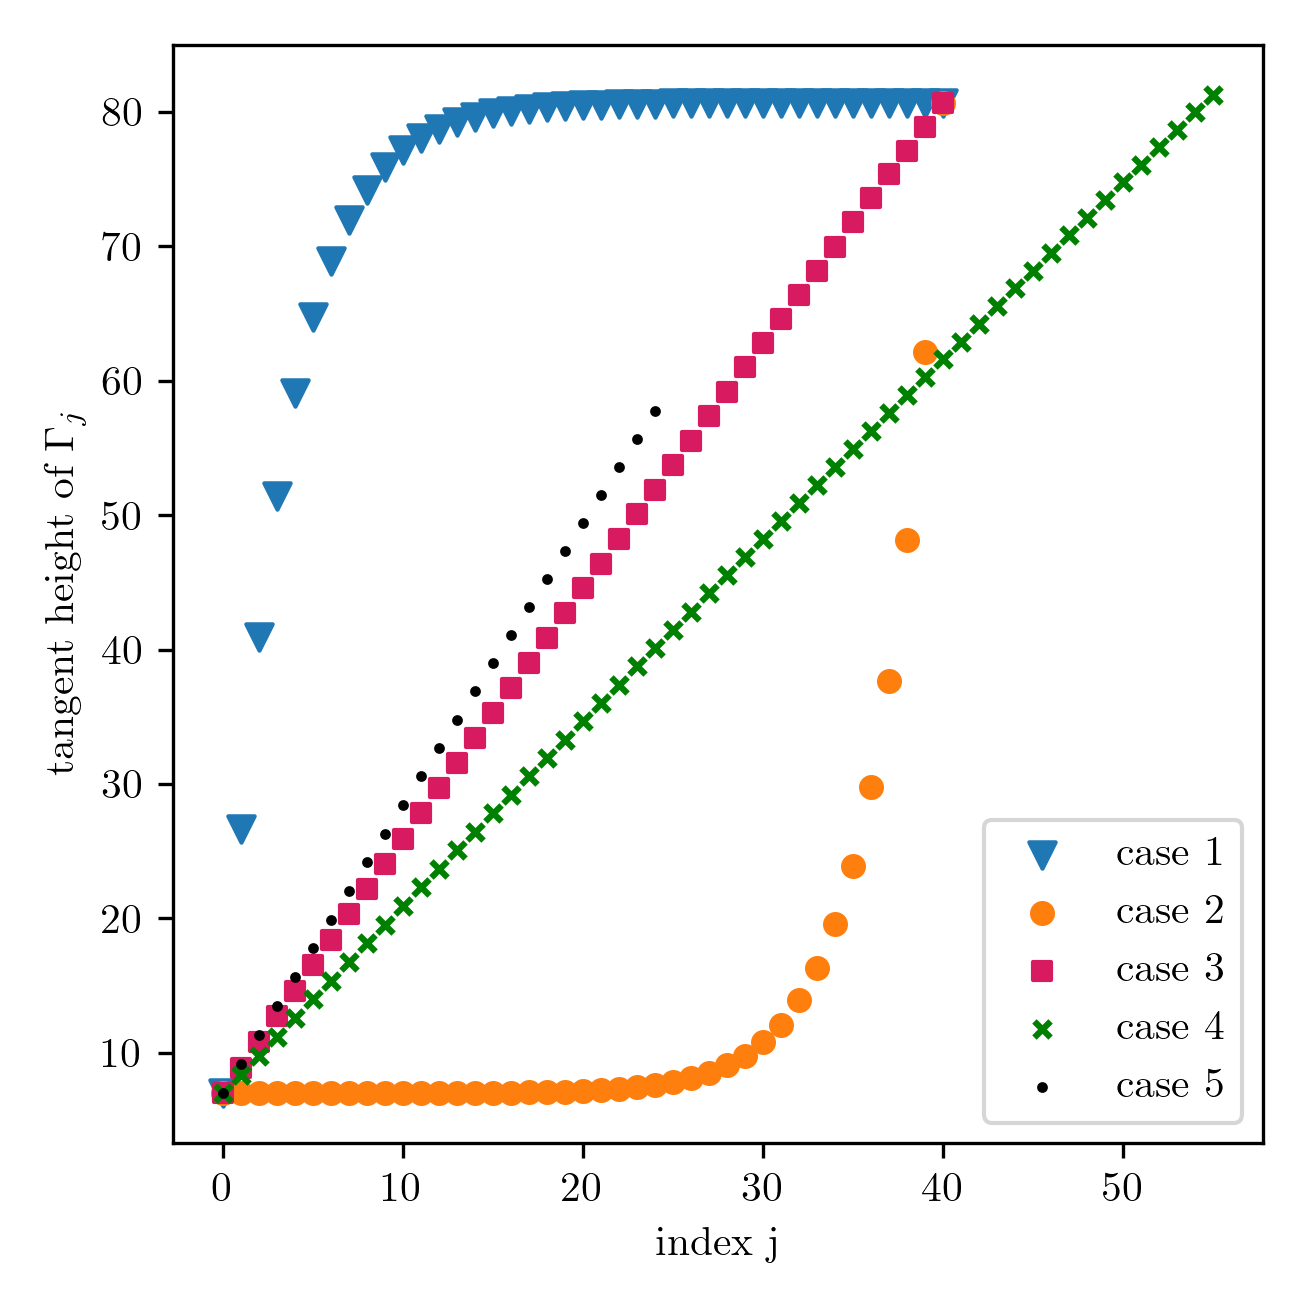
\includegraphics{MeasTangHeight.png}
	\caption[Tangent heights for different sequences of measurements.]{Tangent heights for five different sequences of measurements.}
	\label{fig:TangHCases}
\end{figure}
For five different measurement strategies the tangent heights according to the pointing angles are plotted in Fig.~\ref{fig:TangHCases}.
The measurement test cases are:
\begin{itemize}
	\item[{
\includegraphics[height=0.65\baselineskip]{CASE1.png}}] \textbf{Case 1} includes 42 measurements between heights of $\approx7$km and $\approx83$km with pointing angles
	\begin{align*} 
		\phi_j  = \Bigg(\frac{-1}{1.25^{j-1}} + 1 \Bigg) \phi_{\text{max}} , \qquad  \text{for } j = 1, \dots, 42  \, .
	\end{align*} 
	\item[{
\includegraphics[height=0.65\baselineskip]{CASE2.png}}] \textbf{Case 2} includes 42 measurements between heights of $\approx7$km and $\approx83$km with pointing angles
	\begin{align*} 
		\phi_j  = \frac{1.25 ^{j-1}}{ 1.25 ^{m-1}} 0.99 \phi_{\text{max}},  \qquad  \text{for } j = 1, \dots, 42\, .
	\end{align*}
	\item[{
\includegraphics[height=0.65\baselineskip]{CASE3.png}}] \textbf{Case 3} includes 42 measurements between heights of $\approx 7$km and $\approx 83$km with pointing accuracy $150 \text{arc sec}$ and pointing angles
	\begin{align*} 
		\phi_j  = (j-1) 150 \text{arc sec} ,  \qquad  \text{for } j = 1, \dots, 42\, .
	\end{align*}
	\item[{
\includegraphics[height=0.65\baselineskip]{CASE4.png}}] \textbf{Case 4} includes 83 measurements between heights of $\approx 7$km and $\approx83$km with pointing accuracy $77.5 \text{arc sec}$  and pointing angles
	\begin{align*} 
		\phi_j  =   (j-1) 77.5 \text{arc sec} ,  \qquad  \text{for } j = 1, \dots, 83\, .
	\end{align*}
	\item[{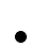
\includegraphics[height=0.65\baselineskip]{CASE5.png}}] \textbf{Case 5} includes 30 measurements between heights of $\approx 7$km and $\approx 68$km with pointing accuracy $175  \text{arc sec}$ and pointing angles
	\begin{align*} 
		\phi_j  =  (j-1) 175 \text{arc sec} ,  \qquad  \text{for } j = 1, \dots, 30\, .
	\end{align*}
\end{itemize} 
Case 1 collects more data in low signal regions at high altitudes.
Case 2 collects more data in high signal regions at low altitudes.
Case 3, case 4, and case 5 measure at equidistantly spaced pointing angles with different pointing accuracies.
The pointing accuracy determines how well the satellite can point in a certain direction and so the spacing of tangent heights in the atmosphere for a satellite at $h_{\text{sat}}$.
Case 1, 2, 3, and 4 measure in between heights $h_{L,1} = 6.9$km and $h_{L,n} = 83.3$km, whereas case 5 does not collect measurements in high altitude regions.
The pointing accuracy for case 3 in Fig.~\ref{fig:TangHCases} of $150\text{arc sec}$ was given to us by the Canberra Space team of the University of New South Wales~\cite{CubeSatInternal}.
Case 4 has half the pointing accuracy of case 3, and case 5 has a slightly larger pointing accuracy than case 3.
We visually assess the effective rank and how the singular values behave to determine which of the test cases is most effective.
More specifically, if the singular values decay fast and only a few singular values lie above an SNR of 150, the forward map is rather uninformative.
If the singular values decay slowly and many singular values lie above an SNR of 150, we classify the forward map as informative.
%\textcolor{red}{Another, they are multiplying like rabbits. Or flies. Which is more annoying?}
%\textcolor{red}{why is this plot here before you defined the cases? That's not remotely OK.}

\begin{figure}[ht!]
	\centering
	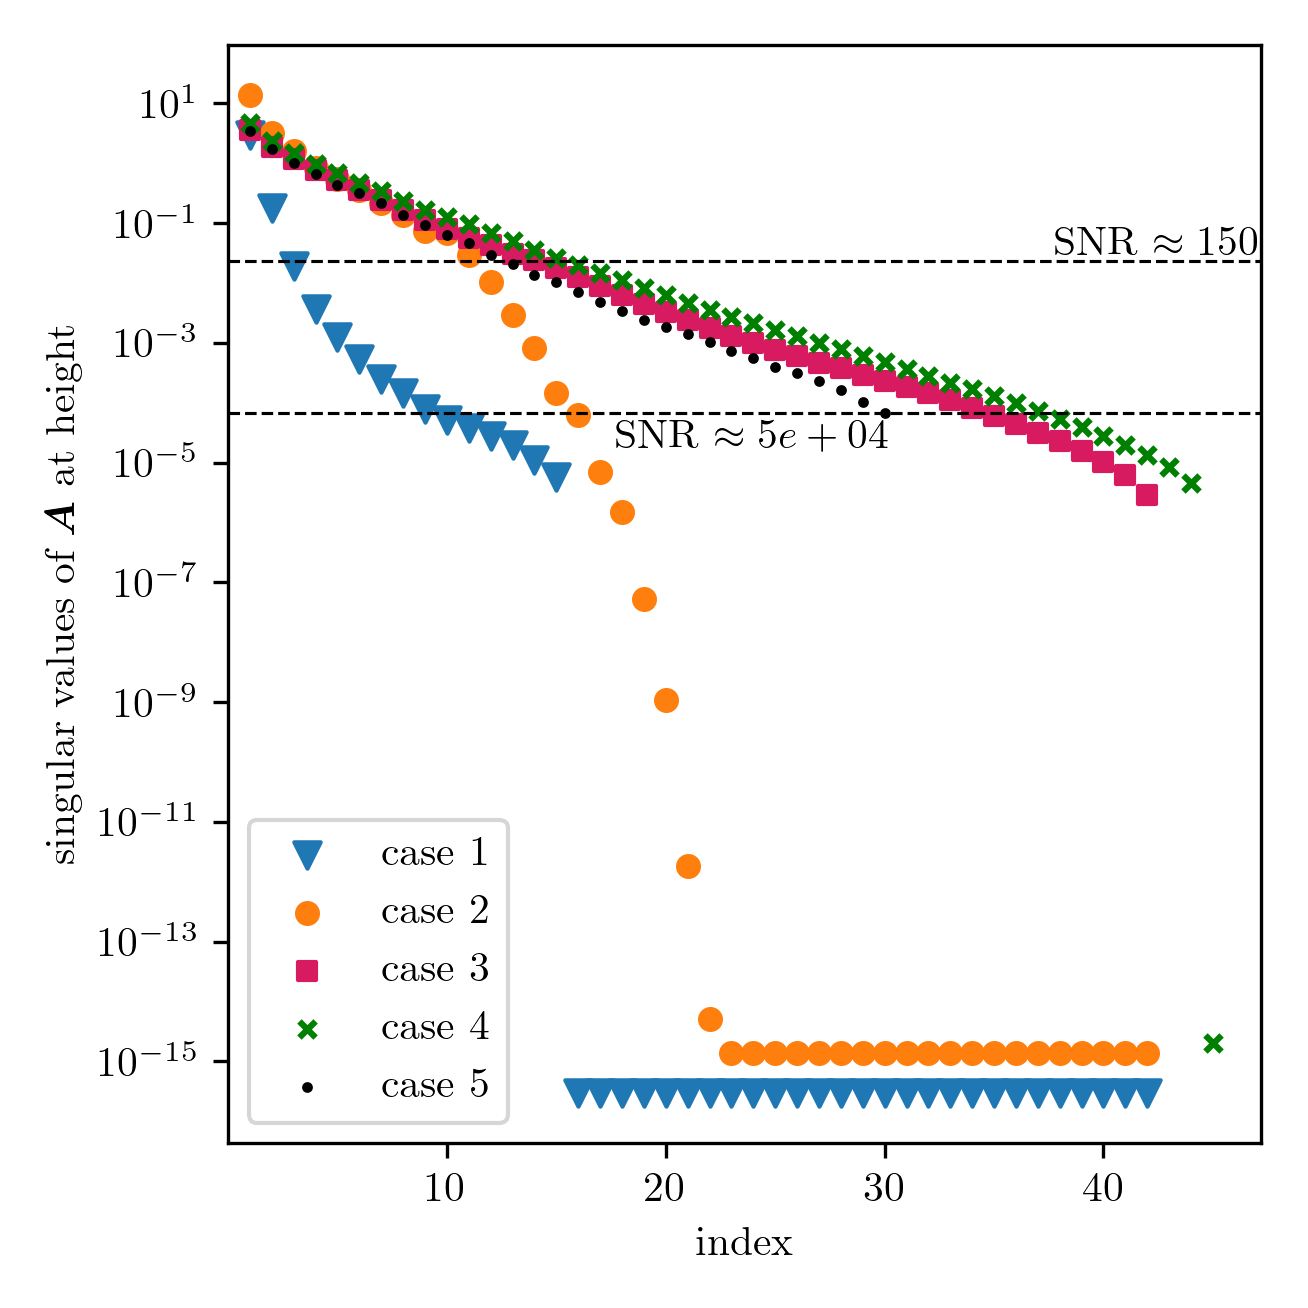
\includegraphics{SingValA.png}
	\caption[Singular values of linear forward model matrix for different sequences of measurements.]{Singular values of the forward model matrix for different sequences of measurements.
	The corresponding tangent heights of the test cases are plotted in Fig.~\ref{fig:TangHCases}. The dotted vertical line marks an SNR according to $\sigma_1$ of measurement case 5.}
\label{fig:SingA}
\end{figure}
In Fig.~\ref{fig:SingA}, we plot the singular values for each of the measurement cases.
The dotted lines in Fig.~\ref{fig:SingA} correspond to an SNR of roughly 150 with respect to the largest singular value of case 5 and an SNR according to the lowest singular value of case 5, which would be required to reconstruct all information provided by the forward model.
The largest singular value of case 5 is similar to the largest singular values of case 1, 3, and 4, so the dotted line for an SNR of $\approx 150$ is indicative for those cases as well.
Fig.~\ref{fig:SingA} shows that case 2 has the largest singular value of all cases but its singular values decrease faster than the singular values of cases 3, 4, and 5 especially below the SNR of 150.
Additionally, case 2 has a smaller effective rank than cases 3, 4, and 5.
The singular values of case 1 are decreasing most rapidly compared to all other cases. Case 1 has the largest number of singular values below an SNR of 150 and the smallest effective rank.
We conclude that neither case 1 nor case 2 is effective.

Cases 3, 4, and 5 with equidistantly spaced pointing angles have similar effective ranks and the singular values do not decrease as quickly compared to case 1 and case 2.
Case 4 measures almost twice as much compared to case 3 but does not provide much more information, which would justify the engineering effort required to achieve such pointing accuracy.
The slightly larger pointing accuracy in case 5 compared to case 3 provides similar information.
The last 5 to 10 singular values of case 3 are so small that the information will be lost due to the noise.
That is why without losing too much crucial information above the SNR of 150 case 5 measures only up to a height of $\approx 68$km instead of $\approx83$km where the data is noise-dominated.
Note, that if one wanted to obtain all information provided by the forward model, an SNR of roughly $10^4$ is required.
%\textcolor{red}{Oh come on, you are showing pictures of singular values without specifying exactly what the forward map and discretization is. That's not acceptable. If these are intended to be indicative, you need to be a damn site clearer about what they represent, and are trying to show.}
%\textcolor{red}{why? Explain your reasoning. If you don't say something specific, quantitative, it's just waffle.}
% \textcolor{red}{where is this spacing? At the satellite? A spacing in time? On the planet Mars. Be specific. All the way through, you need to tighten up loose statements like this.}
% 
%The corresponding singular values are plotted in Fig.~\ref{fig:SingA}, of which the first 25 decrease linearly in log-space and about 10-15 singular values lie above the SNR. \textcolor{red}{where is this spacing? At the satellite? A spacing in time? On the planet Mars. Be specific. All the way through, you need to tighten up loose statements like this.}
%In comparison, if we measure a lot of times in regions where the data is noise-dominated (high altitude), case 1, we do obtain more information since the singular values decrease rapidly.
%\textcolor{red}{Oh come on, you are showing pictures of singular values without specifying exactly what the forward map and discretisation are. That's not acceptable. If these are intended to be indicative, you need to be a damn site clearer about what they represent, and are trying to show.}
%Measuring lots of times at low altitudes, where the data is informative, and less at higher altitudes, case 2, does not seem optimal either, as we observe one larger singular value, but the other singular values decrease faster compared to case 3.
%Now consider case 4, where we double the number of measurements compared to case 3. We do get slightly larger singular values, but not so significantly that it would be worth the engineering effort required to achieve that.
%The measurements with equidistance-spaced tangent height seem to be most effective. \textcolor{red}{why? Explain your reasoning. If you don't say something specific, quantitative, it's just waffle.}
%By exploratory analysis, we find that we can tolerate a slightly larger distance between tangent heights (pointing accuracy of $175\text{arc sec}$) than required by~\cite{CubeSatInternal}, see case 5.
%In that case, we also stop measuring when the signal is too noisy and decrease the number of measurements taken without losing crucial information.
%We note that if one wanted to obtain all information provided by the forward model, we would need a signal-to-noise ratio of roughly $10^7$.
%\textcolor{red}{on the contrary - -you have just been arguing that it does matter. no, this makes sense if the goal is to reduce noise.}
%This contradicts the current measurement setup on the AURA MLS~\cite{livesey2006retrieval}, which reports high noise in lower atmospheric regions, due to thermal radiation from the earth, and measures more in those regions.
%\textcolor{red}{oh no, I had hpped this section would be 'we' free.}
%\textcolor{red}{where do you explain why this SNR has a line here?,
	%Were is the clear definition of these cases? I could not find it.}

In principle, this shows that it does matter how one measures, but the forward model does not provide more information by measuring more in regions where the information content is low or high.
The test cases show that an efficient measurement strategy may consist of equidistantly spaced pointing angles and does stop measuring when the singular values are too low. 
Consequently, we proceed with case 5.
Next, the right singular vectors of the forward model will be assessed to see to which parameter structures within the atmosphere our model is sensitive to.

\begin{figure}[ht!]
	\centering
	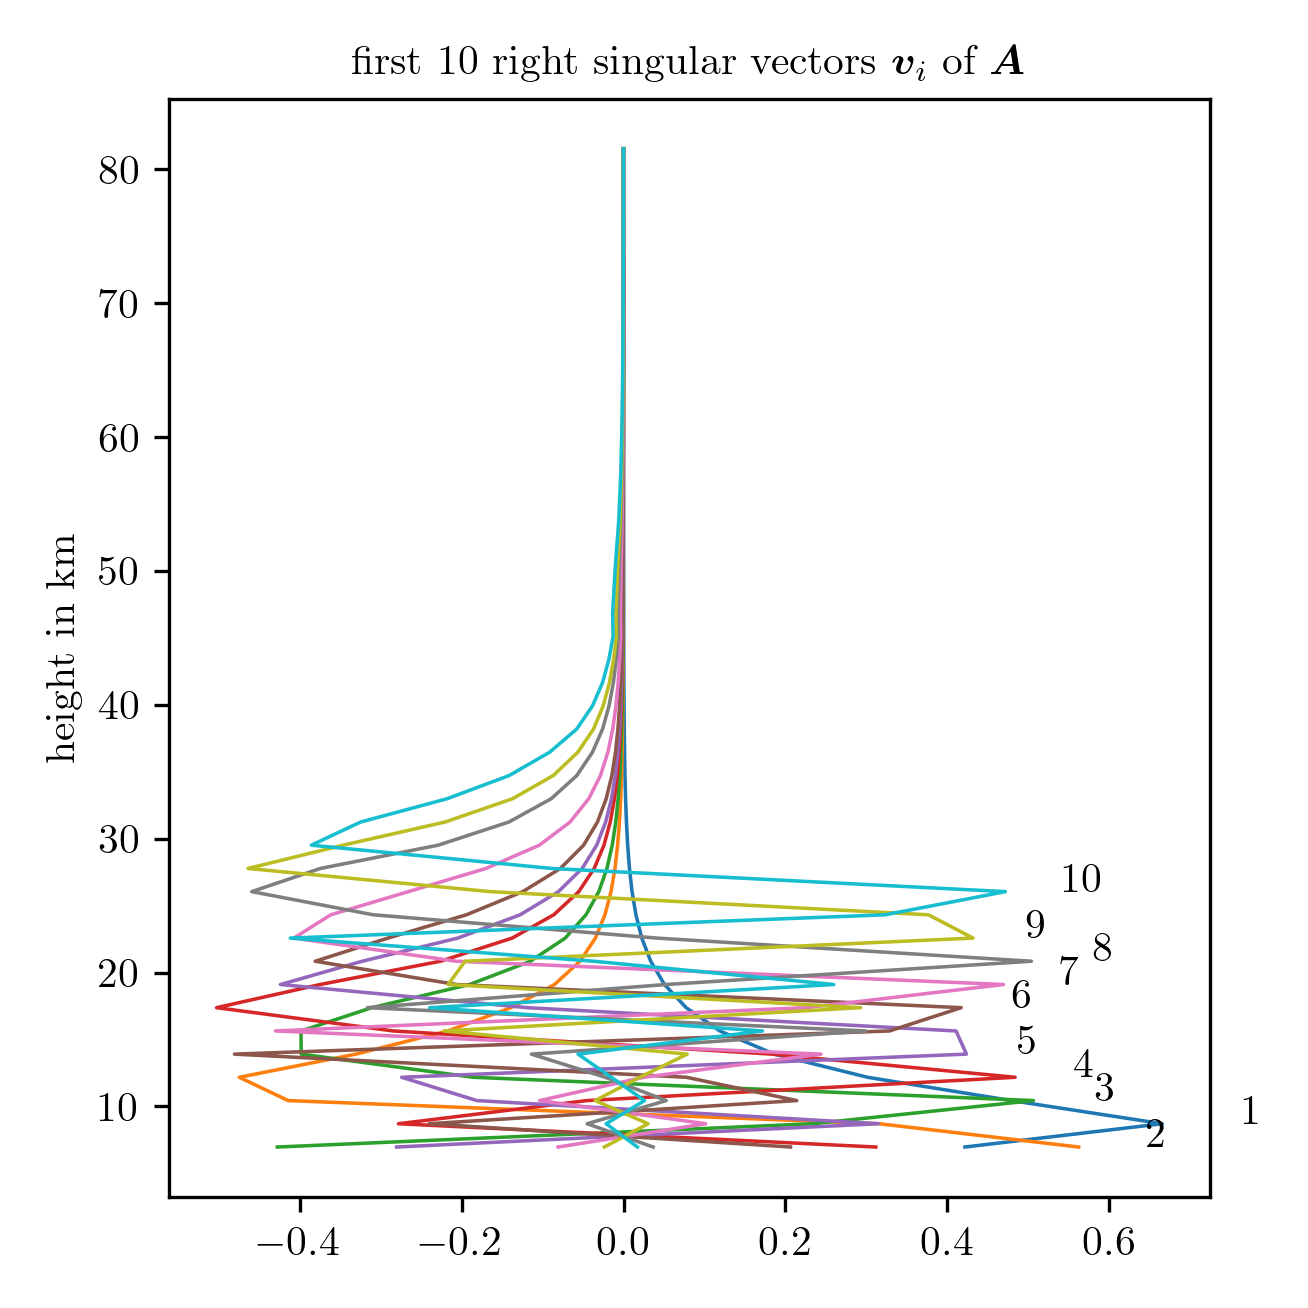
\includegraphics{SingVecA.png}
	\caption[First 10 right singular vectors of forward model.]{First 10 right singular vectors of the forward model matrix $\bm{A}_L$ for measurements case 5 in Fig.~\ref{fig:TangHCases}. These singular vectors correspond to high singular values of the forward model in Fig.~\ref{fig:SingA}.}
	\label{fig:SingVecA}
\end{figure}
\begin{figure}[ht!]
	\centering
	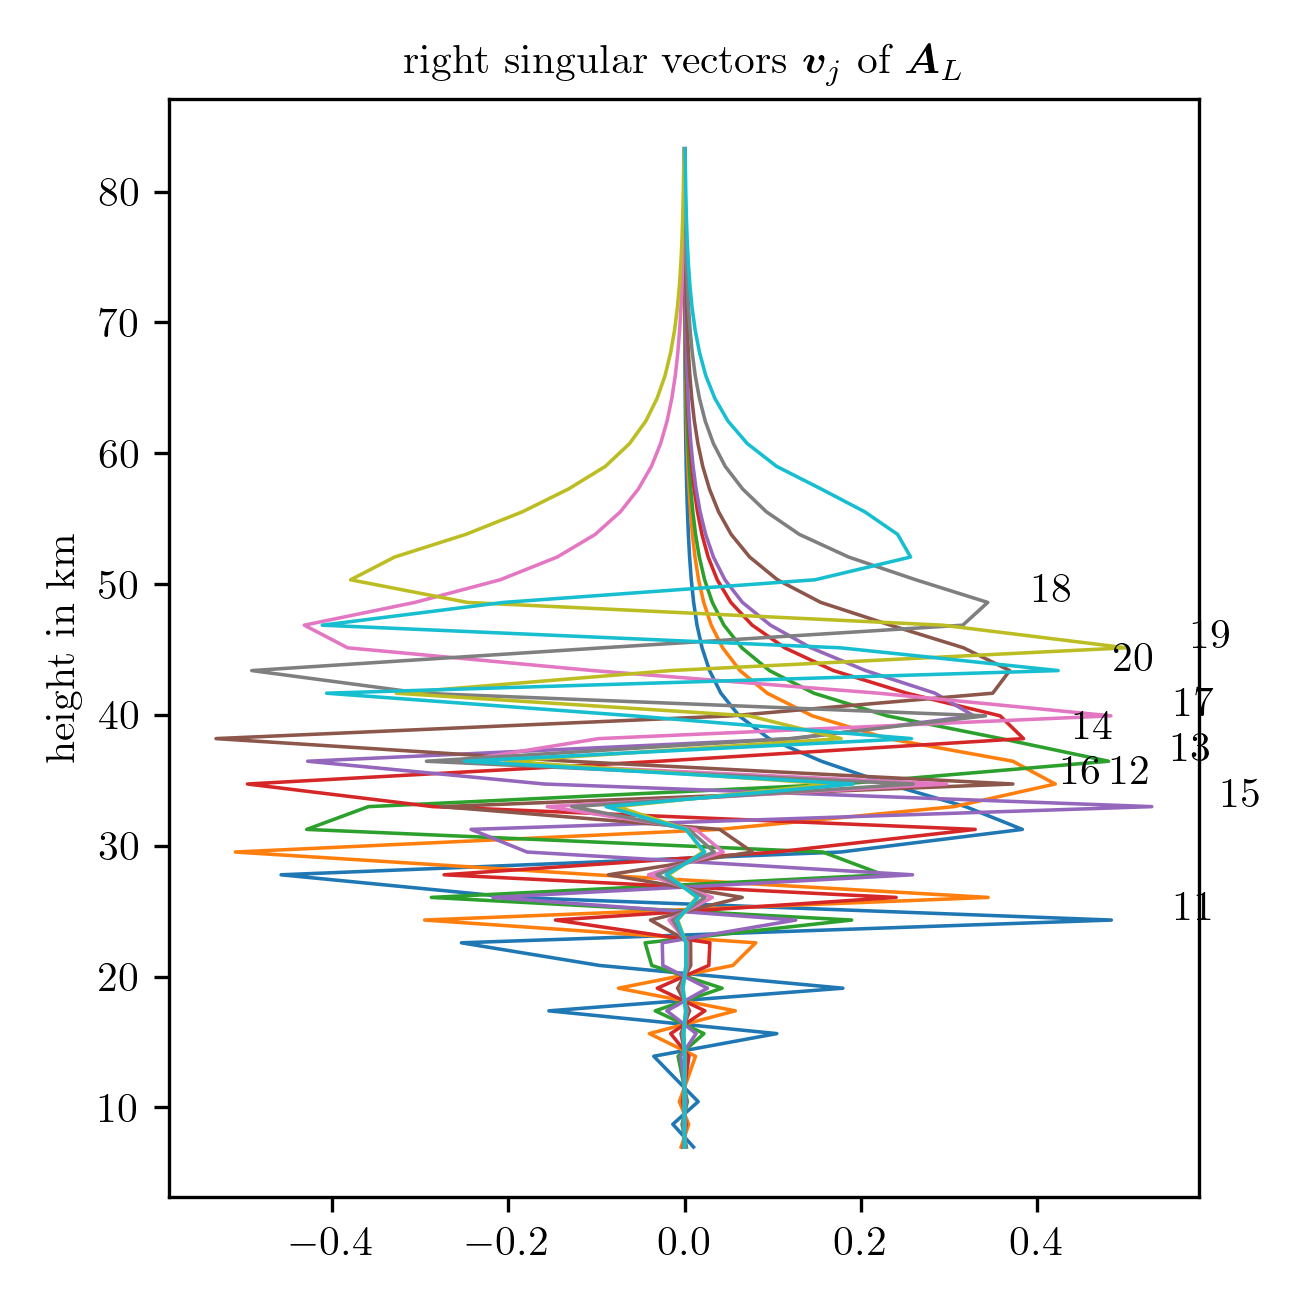
\includegraphics{MiddleVecA.png}
	\caption[Right singular vectors 11 to 19 of forward model.]{Right singular vectors with index $j = 11,\dots, 200$ of the forward model matrix $\bm{A}_L$ for measurements case 5 in Fig.~\ref{fig:TangHCases}.
		These singular vectors correspond to singular values in Fig.~\ref{fig:SingA}, where the noise level is similar to the data.}
	\label{fig:middleSpace}
\end{figure}
\begin{figure}[ht!]
	\centering
	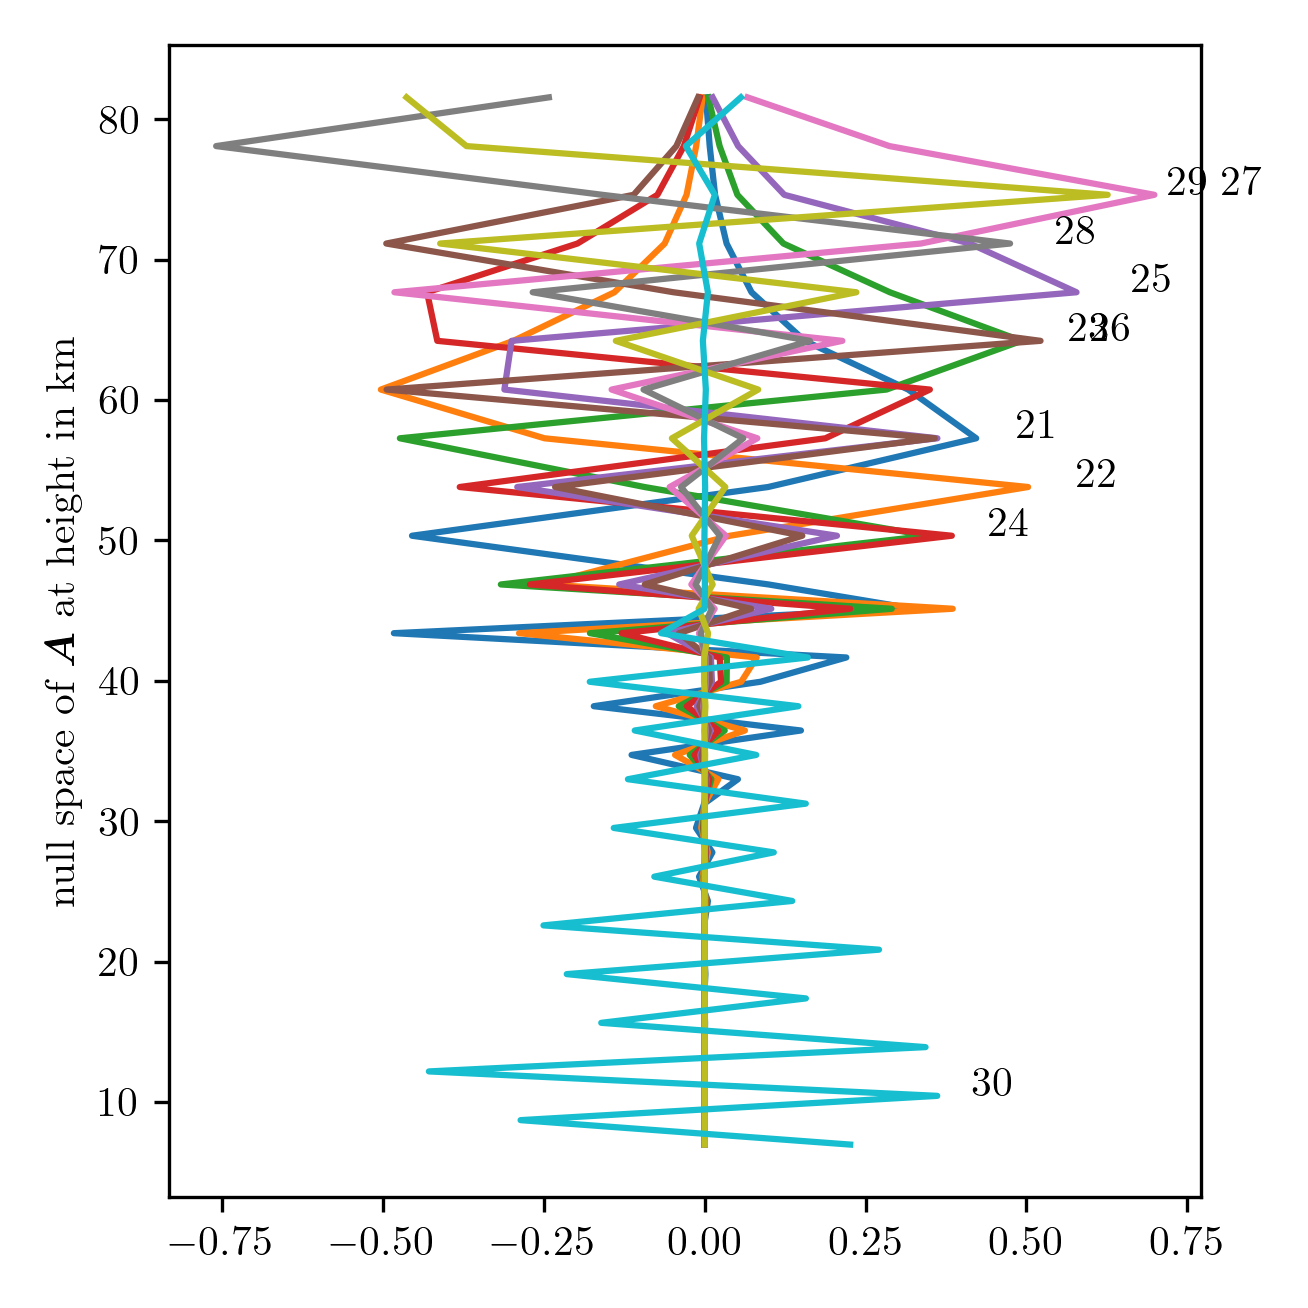
\includegraphics{NullVecA.png}
	\caption[Last 10 right singular vectors of forward model.]{Last 10 right singular vectors of the forward model matrix $\bm{A}_L$ for measurements case 5 in Fig.~\ref{fig:TangHCases}. These singular vectors correspond to small singular values of the forward model in Fig.~\ref{fig:SingA}, where the data is noise-dominated.}
	\label{fig:nullSpace}
\end{figure}
The parameter space of $\bm{A}_L$ spanned by the first 10 right singular vectors, corresponding to the 10 largest singular values in Fig.~\ref{fig:SingA}, is plotted in Fig.~\ref{fig:SingVecA}.
These right singular vectors represent parameter structures in the lower atmospheric regions.
So we can assume that, given some data, we will be able to provide good reconstructions of the parameter in lower altitudes up to $\approx30$km.
The right singular vectors in Fig.~\ref{fig:middleSpace} correspond to the singular values $\sigma_j$ for $j = 11, \dots, 20$ around the SNR of 150 (see Fig.~\ref{fig:SingA}).
This is roughly where the noise starts to dominate the data.
The parameter space spanned by those right singular vectors represents parameter values in the middle atmosphere.
Consequently, we expect an increasing uncertainty of reconstructed parameter values at heights between $\approx20$km and $\approx50$km.
The right singular vectors in Fig.~\ref{fig:nullSpace} corresponding to the smallest 10 singular values span structures in parameter space at higher altitudes, and the associated data space is noise-dominated.
That is why we will not be able to reconstruct parameter values from the ground truth above $\approx50$km.
More specifically, the retrieved parameter values at higher altitudes will have large uncertainties and will be determined by the prior or, in the case of a regularisation approach, by the regulariser~\cite{tan2016LecNot}.
\clearpage
%The difference in between tangent heights is between 2.05km and 2.17km.
% \textcolor{red}{Actually, you should calculate this from the MIPAS specifications, or similar. It claims 1-3km resolution, presumably at a distance of 500km. So, what's that in arc seconds? It's also related to your vertical discretization, or, more to the point, your vertical discretization is determined by this.}
%  around the SNR,


Finally, the data vector $\bm{y} = \bm{A}(\bm{x}) + \bm{\eta} $ is computed according the RTE (see Eq.~\ref{eq:RTE} and Eq.~\ref{eq:absRTE}) and the froward model is determined by the data collection strategy of case 5, with $m = 30$ measurements between $\approx 7$km and $\approx 68$km and a satellite pointing accuracy of $175\text{arc sec}$ (see in Fig.~\ref{fig:TangHCases}).
% according to the RTE as in Eq.~\ref{eq:RTE} and Eq.~\ref{eq:absRTE} using the trapezoidal integration rule.
As already mentioned, we set the SNR to 150 and plot the data in Fig.~\ref{fig:DataPlot}, which is noise-dominated in higher altitudes.
Given the data, we aim to determine the posterior distributions over ozone $\bm{x}$, pressure $\bm{p}$ and temperature $\bm{T}$.
\begin{figure}[h!]
	\centering
	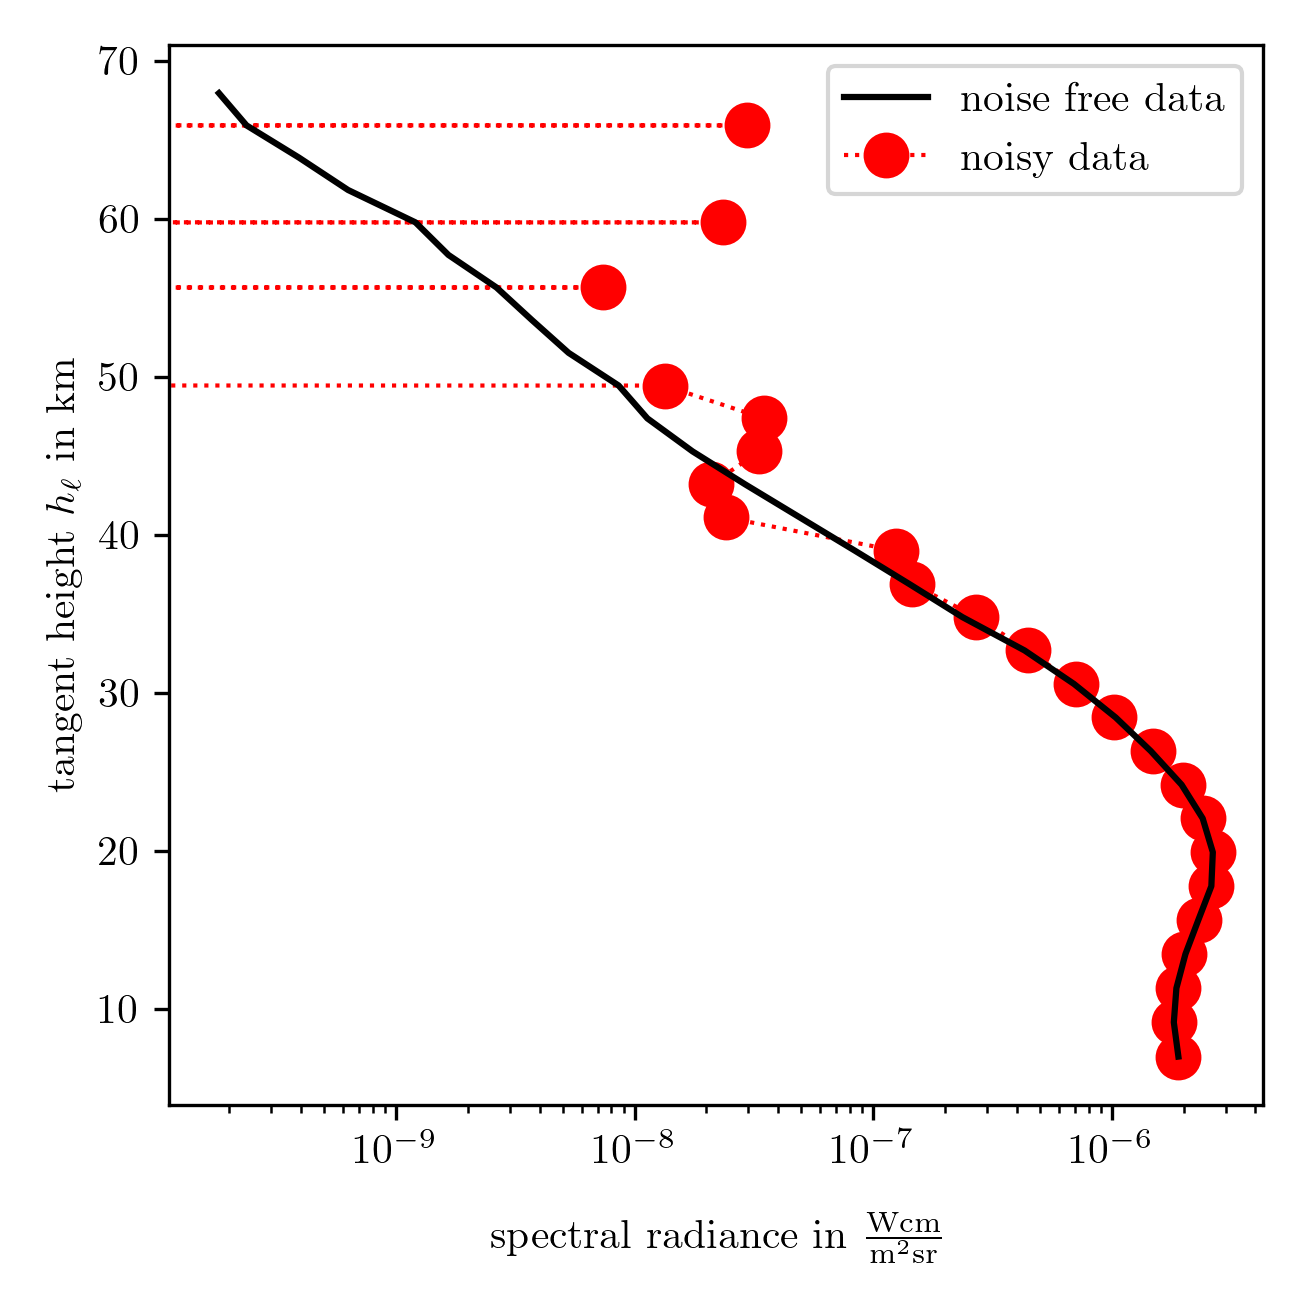
\includegraphics{DataPlot.png}
	\caption[Logarithmic plot of the data points at different tangent height.]{Logarithmic plot of data points at different tangent height. Note that negative values are not plotted, and noise is dominating at higher altitudes.}
	\label{fig:DataPlot}
\end{figure}
\clearpage
